\documentclass[a4paper]{article}
\usepackage[T1]{fontenc}
\usepackage{amsmath}
\usepackage{amsthm}
\usepackage{amssymb}
\usepackage{float}
\usepackage[utf8]{inputenc}
\usepackage{graphicx}
\usepackage[italian]{babel}
\usepackage{thmtools}
\newtheorem{theorem}{Theorem}
\newtheorem*{definition}{Definition}
\newtheorem{example}{Example}

\begin{document}

\author{Lorenzo Dentis, lorenzo.dentis@edu.unito.it}
\title{Esercizio 1}
\maketitle

\section{logica proposizionale}
\subsection{Esercizio 1}
Which of the following propositional formulas represents the sentence, 'He will come on the 8:15 or the 9:15 train; if the former, he will have time to visit us', where
\begin{itemize}
	\item p means 'He will come on the 8:15'
	\item q means 'He will come on the 9:15'
	\item r means 'He will have time to visit us'
\end {itemize}
Risposta 5: $(p \lor  q) \land (p \rightarrow r)$
\subsection{Esercizio 2}
Which of the following sentences has the logical form $(p \land q) \rightarrow r$ ?\\
Risposta 3: If inflation is up and an election is approaching, then public borrowing goes up.
\subsection{Esercizio 3}
Which of the following propositional formulas is satisfied by the valuation which assigns T to P, and F to q and r.\\
Risposta 2: $\lnot ( \lnot r \rightarrow ( p \land q))$
\subsection{Esercizio 4}
Which of the following propositional formulas is a tautology?\\
Risposta 5: $ (p \leftrightarrow q) \land (p \leftrightarrow \lnot q)$
\subsection{Esercizio 5}
Which of the following entailments is valid?\\
Risposta 2: $ p, \lnot p \leftrightarrow q \models \lnot q $
\subsection{Esercizio 6}
Risposta 3:
\begin{displaymath}
\begin{array}{|c c c|c|}
p & q & r & (p \rightarrow q) \lor \lnot (r \land \lnot q) \\
\hline 
T & T & T & T \\
T & T & F & T \\
T & F & T & F \\
T & F & F & T \\
F & T & T & T \\
F & T & F & T \\
F & F & T & T \\
F & F & F & T \\
\end{array}
\end{displaymath}
\subsection{Esercizio 7}
Which of the following formulas represents the sentence 'If Smith has installed central heating, then he has sold his car or he has not paid his mortage', where:
\begin{itemize}
	\item p means 'Smith has installed central heating'
	\item q means 'Smith has sold his car'
	\item r means 'Smith has paid his mortage'.
\end{itemize}
Risposta 4: $ p \rightarrow q \lor \not r $
\subsection{Esercizio 8}
Which of the following formulas represents the sentence, 'Share prices will go up, and if interest rates go up too, there will be a recession', where:
\begin{itemize}
	\item p means 'share prices will go up'
	\item q means 'interest rates will go up'
	\item r means 'there will be a recession'.
\end{itemize}
Risposta 1: $p \land q \rightarrow r $
\subsection{Esercizio 9}
Which of the following sentences could be written as $ p \lor (q \land r)$, for suitable p, q, and r ?\\
Risposta 2 : You can go swimming, or use the sauna and the shower.
\subsection{Esercizio 10}
According to the standard convention about binding priorites, the formula, $ \lnot p \rightarrow \lnot q \land r $, is implicity one of the following. Which?\\
Risposta 4: $ ( \lnot p) \rightarrow (( \lnot q) \land r) $
\subsection{Esercizio 11}
Which of the following formulas has the parse tree:\\
\begin{figure}[H]
	\centering
	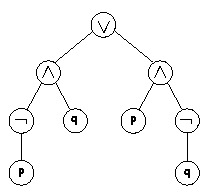
\includegraphics[scale = 0.5]{parsetree.jpg}
\end{figure}
Risposta 1: $ ( \lnot p \land q) \lor (p \land \lnot q) $

\section{notazioni e definizioni}
\subsubsection{Insiemi}
notazione per Naturali $ \mathbb{N} $, Interi $ \mathbb{Z} $, Reali $ \mathbb{R} $, elemento contenuto in un insieme $ \in $
\newline
\begin{definition}[Intersezione]L'intersezione ($\cap$) tra due insiemi $A$ e $B$ è l'insieme degli elementi che appartengono contemporaneamente sia ad $A$ che a $B$
\end{definition}
\begin{definition}[Unione]L'unione $\cup$ tra due insiemi $A$ e $B$ è l'insieme degli elementi che appartengono ad $A$, a $B$ o ad entrambi.
\end{definition}
\begin{definition}[Differenza]La differenza $\setminus$ tra due insiemi $A$ e $B$, indicata con $A \setminus B$ è l'isieme degli elementi di $A$ esclusi gli elementi che appartengono anche a $B$
\end{definition}
\begin{definition}[Power Set]L' insieme potenza (power set) $\mathcal{P}$($A$) è l'insieme di tutti i sottoinsiemi di $A$. $\mathcal{P}(A)=\{X : X \subseteq A\}$ 
\end{definition}
\begin{definition}[Complemento]L'insieme complemento di un inseme $A$, scritto $A^{C}$, è l'insieme ottenuto dalla differenza tra l'insieme Universo ed $A$. $A^{C} = U \setminus A$
\end{definition}
\begin{definition}[Sottoinsieme]Un sottinsieme $ \subset $ di $A$ è un insieme che contiene solamente elementi contenuti in $A$.
\end{definition}
\begin{definition}[Sottoinsieme stretto]Un sottinsieme stretto $ \subseteq $  di $A$ è un insieme che contiene solamente gli elementi contenuti in $A$, eventualmente tutti.
\end{definition}

\subsubsection{relazioni}
\begin{definition}[Prodotto Cartesiano]Il prodotto cartesiano di due insiemi $A$ e $B$ è l'insieme delle coppie ordinate $(a,b)$ con $a \in A$ e $b \in B$ Formalmente:\\
$A\times B:=\{(a,b):a\in A\;{\mathrm  {e}}\;b\in B\}$ 
\end{definition}
\begin{definition}[Relazione binaria]
Si definisce relazione binaria $R$ tra due insiemi non vuoti $A$ e $B$ un sottoinsieme di $ A \times B$. Due elementi $x$ e $y$ sono messi in relazione da $R$ se: 
$(x,y)\in R\ $ ed in tal caso si scrive $xRy$.
\end{definition}
\begin{definition}[Relazione riflessiva]
Una relazione binaria $R$ in un insieme $X$ è detta riflessiva se ogni elemento di $X$ è in tale relazione con sé stesso.
In simboli: $R$ è riflessiva se: $ \forall a\in X,\ aRa.$
\end{definition}
\begin{definition}[Relazione simmetrica]Una relazione binaria $R$ in un insieme$ X $è simmetrica se e solo se, presi due elementi qualsiasi $a$ e $b$, vale che se $a$ è in relazione con $b$ allora anche $b$ è in relazione con $a$.\\
In simboli: $\forall a,b\in X,\ aRb\Rightarrow bRa$
\end{definition}
\begin{definition}[Relazione transitiva]Una relazione transitiva $R$ in un insieme $X$ è transitiva se e solo se prendendo tre elementi qualsiasi $a$, $b$ e $c$ $ \in X$, tali che $aRb$ e $bRc$ allora $aRc$
\end{definition}
\begin{definition}[Relazione di equivalenza]Una relazione di equivalenza $R$ su $A$ è una relazione riflessiva, simmetrica e transitiva.
\end{definition}
\begin{definition}[Chiusura transitiva di una relazione]Data una relazione $R$ su $A\times A$ chiamiamo chiusura transitiva di $R$, e la indichiamo con $R^{+}$ la seguente relazione:\\
	$ R^{+} = \{ x, y : 
\end{definition}
	Funzione
 Funzione  di arietà n,
 funzione iniettiva,
 funzione suriettiva,
 funzione biiettiva
\subsubsection{Stringhe e linguaggi}
\subsubsection{Grafi}
\subsubsection{Matrici}
\end{document}
